\documentclass[a4paper,11pt]{article}
\usepackage[german,italian]{babel}
\usepackage{fancyhdr}


\textwidth16cm \textheight24cm \topmargin0mm \headheight0mm
\headsep5mm \oddsidemargin0mm \evensidemargin0mm
\parindent0mm




\usepackage{amsmath}
\usepackage{parskip}
\usepackage{dsfont}
\usepackage{fullpage}
\usepackage{amssymb}
\usepackage{tikz,pgfplots}
\usepackage{cancel}
\usepackage{lmodern}

\usepackage[T1]{fontenc}

\usepackage{theorem}
\usepackage{psfrag}
\usepackage{color}
\usepackage{graphicx}
\usepackage{hyperref}

\usepackage{background}
\usepackage{keystroke}
\usepackage{etoolbox}
\usepackage{subfig}


\makeatletter
\patchcmd{\tableofcontents}{\@starttoc{toc}}{\hypertarget{totoc}{}\@starttoc{toc}}{}{}
\makeatother

\SetBgScale{1}
\SetBgAngle{0}
\SetBgColor{black}
\SetBgPosition{current page.south}
\SetBgVshift{20pt}
\SetBgContents{\tikz[remember picture,overlay]
    \node[inner sep=0pt] {\hyperlink{totoc}{\Return}};}





\hypersetup{
    colorlinks=true,
    linkcolor=black,
    urlcolor=blue,
    pdftitle={Fourier Analysis Documentation},
    pdfpagemode=FullScreen,
}






\begin{document}




\title{Matematica}

\author{Massimiliano Ferrulli}
\date{03.05.2022}



\maketitle

\section*{Coniche}
Studio di coniche, ellissi, paraboliche e iperboli

\pagebreak




\tableofcontents





\pagebreak















\section{Le Coniche }
\subsection{Sezioni coniche}
Nello spazio consideriamo due rette \textit{g} e \textit{a} incidenti nel punto V, con \( \omega \) che è l'angolo generato dall'intersezione delle due rette. 
La rotazione della retta \textit{g} attorno ad \textit{a} genera una superficie illimitata detta cono di rotazione a due falde.






\subsection{Definizione}
Una curva ottenuta come intersezione di un cono di rotazione con un piano \( \alpha \), che non passi per il vertice, è detta conica non degenere
si distinguono 3 casi a dipendenza dell'angolo di incidenta S del piano \( \alpha \) rispetto all'asse \textit{a}. 

Queste curve ottenute come sezioni di un cono, possono essere caratterizzate come luoghi geometrici, cioè come insieme di punti di un piano che soddisfano una condizione geometrica.
 




\subsubsection{Caso 1}
se il piano interseca una sola falda e taglia tutte le generatrici, cioè se \( \delta > \omega \) si ottiene una curva chiusa detta ellisse. 
In particolare se \( \alpha \perp a \) oppure \( \vec{\eta}_\alpha \backslash \backslash \, \vec{v}_a \)   \( (\delta = \frac{\pi}{2}) \) si ottiene una circonferenza
\begin{center}
\begin{minipage}{8cm}
    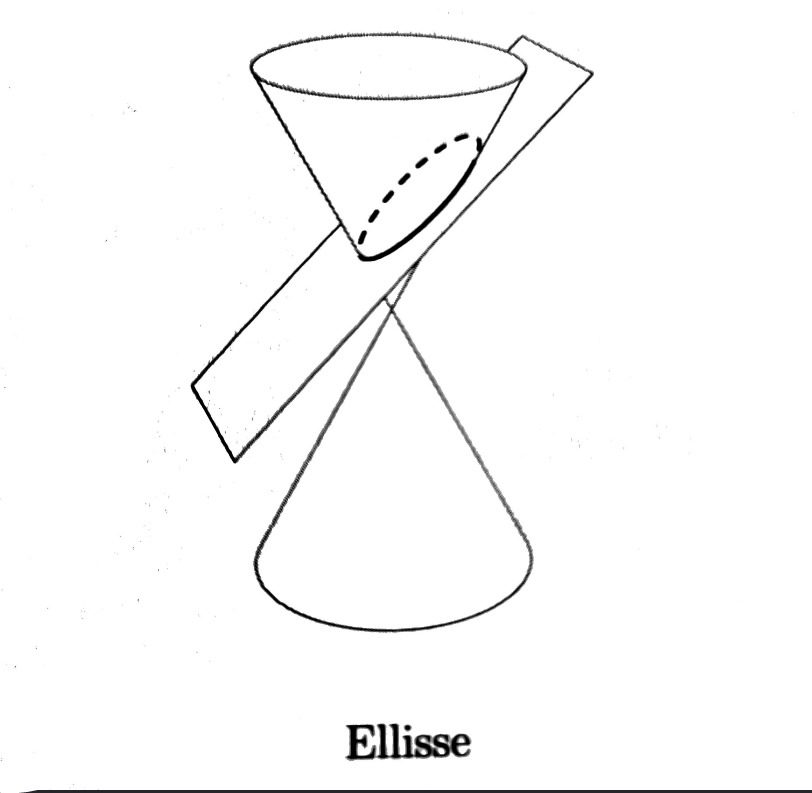
\includegraphics[scale=0.3]{ellisse.png}
\end{minipage}
\end{center}
\paragraph{Luogo geometrico Ellisse}
un'ellisse è l'insieme di punti per i quali la somma delle distanze da due punti \(F_1 e F_2\) (detti fuochi) è costante.





\subsubsection{Caso 2}
se il piano \( \alpha \) interseca una sola falda ed è parallelo ad una generatrice \( ( \delta = \omega) \) si ottiene una curva aperta detta parabola
\begin{center}
\begin{minipage}{8cm}
    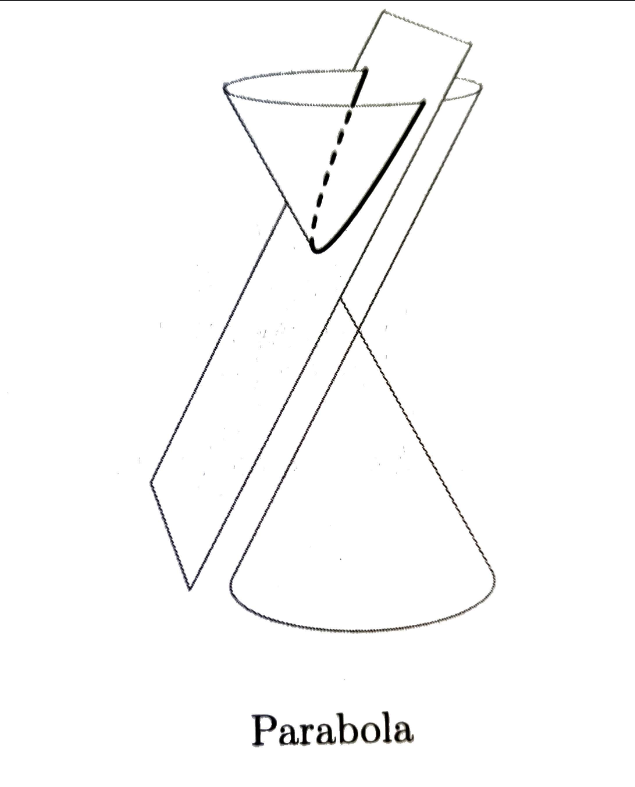
\includegraphics[scale=0.3]{parabola.png}
\end{minipage}
\end{center}
\paragraph{Luogo geometrico Parabola}
è l'insieme dei punti del piano equidistanti da un punto fisso F detto fuoco e da una retta fissa D detta direttrice






\subsubsection{Caso 3}
\begin{center}
\begin{minipage}{8cm}
    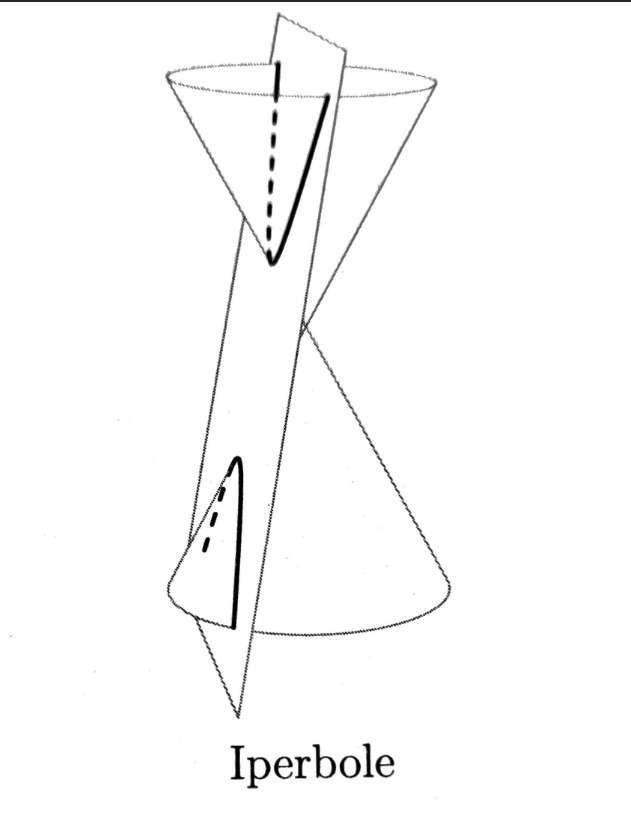
\includegraphics[scale=0.3]{iperbole.png}
\end{minipage}
\end{center}
\(  \delta < \omega \)



\paragraph{Luogo geometrico Iperbole}
È l'insieme dei punti del piano \( \alpha \) per i quali il valore assoluto della differenza delle distanze dai due punti fissi \( F_1 e F_2\) (fuochi) è costante.
  

\paragraph{Ragionamento sulle caratterizzazioni delle coniche}
Queste caratterizzazioni delle coniche come luoghi geometrici del piano sono conseguenze delle loro definizioni come sezioni del cono.
Esaminiamo il caso dell'ellisse, dato dall'intersezioni del piano \( \alpha \) con il cono

\begin{minipage}{8cm}
    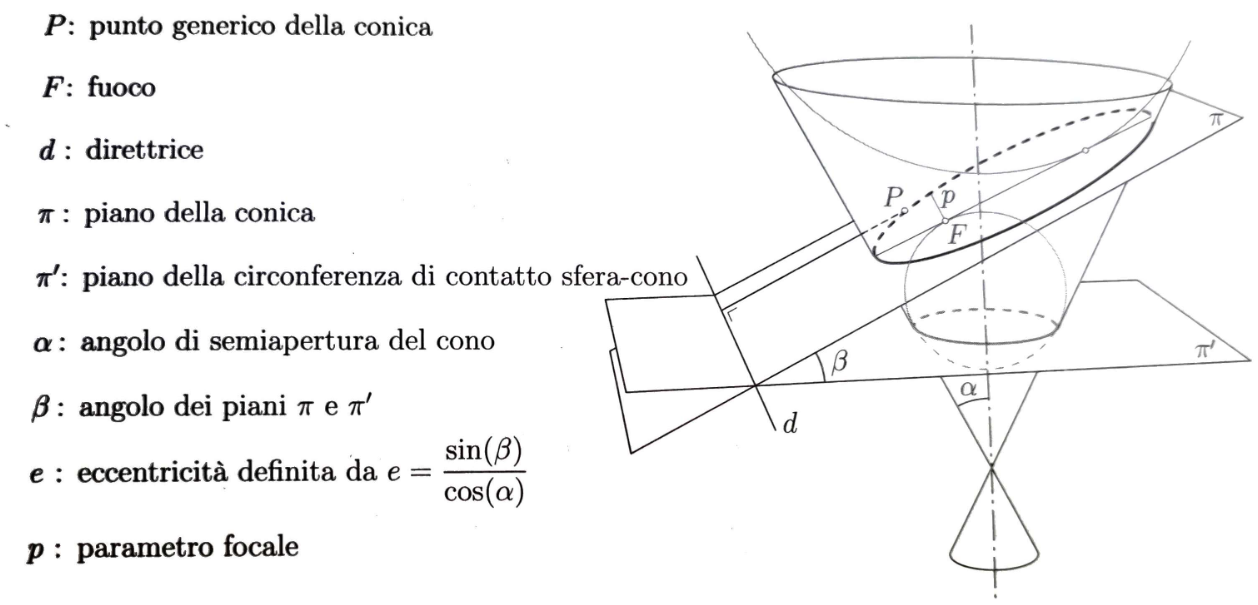
\includegraphics[scale=0.5]{rag_ellisse.png}
\end{minipage}
\\
Si considerino 2 \href{https://it.wikipedia.org/wiki/Sfere_di_Dandelin}{Sfere di Dandelin} tangenti sia al cono \hspace{4mm} (lungo due circonferenze parallele \(C_1 e C_2\) ) che al piano \( \alpha \) (nei punti \(F_1 e F_2\) ) ( i 2 fuochi).
\\
Sia P un punto qualsiasi dell'ellisse, vogliamo dimostrare che \(   \left\lvert PF_1 \right\rvert  + \left\lvert PF_2 \right\rvert    \) è costante cioè dipende dalla scelta di P. La generatrice passante per P interseca le 2 circonferenze nei punti \( A_1 e A_2 \).
Essendo \( c_1 \) parallela a \(c_2\) la distanza \(A_1 A_2\) è costante e indipendente dalla scelta di P.
\\
\begin{figure}[!tbp]
        \centering
        \begin{minipage}[b]{0.4\textwidth}
          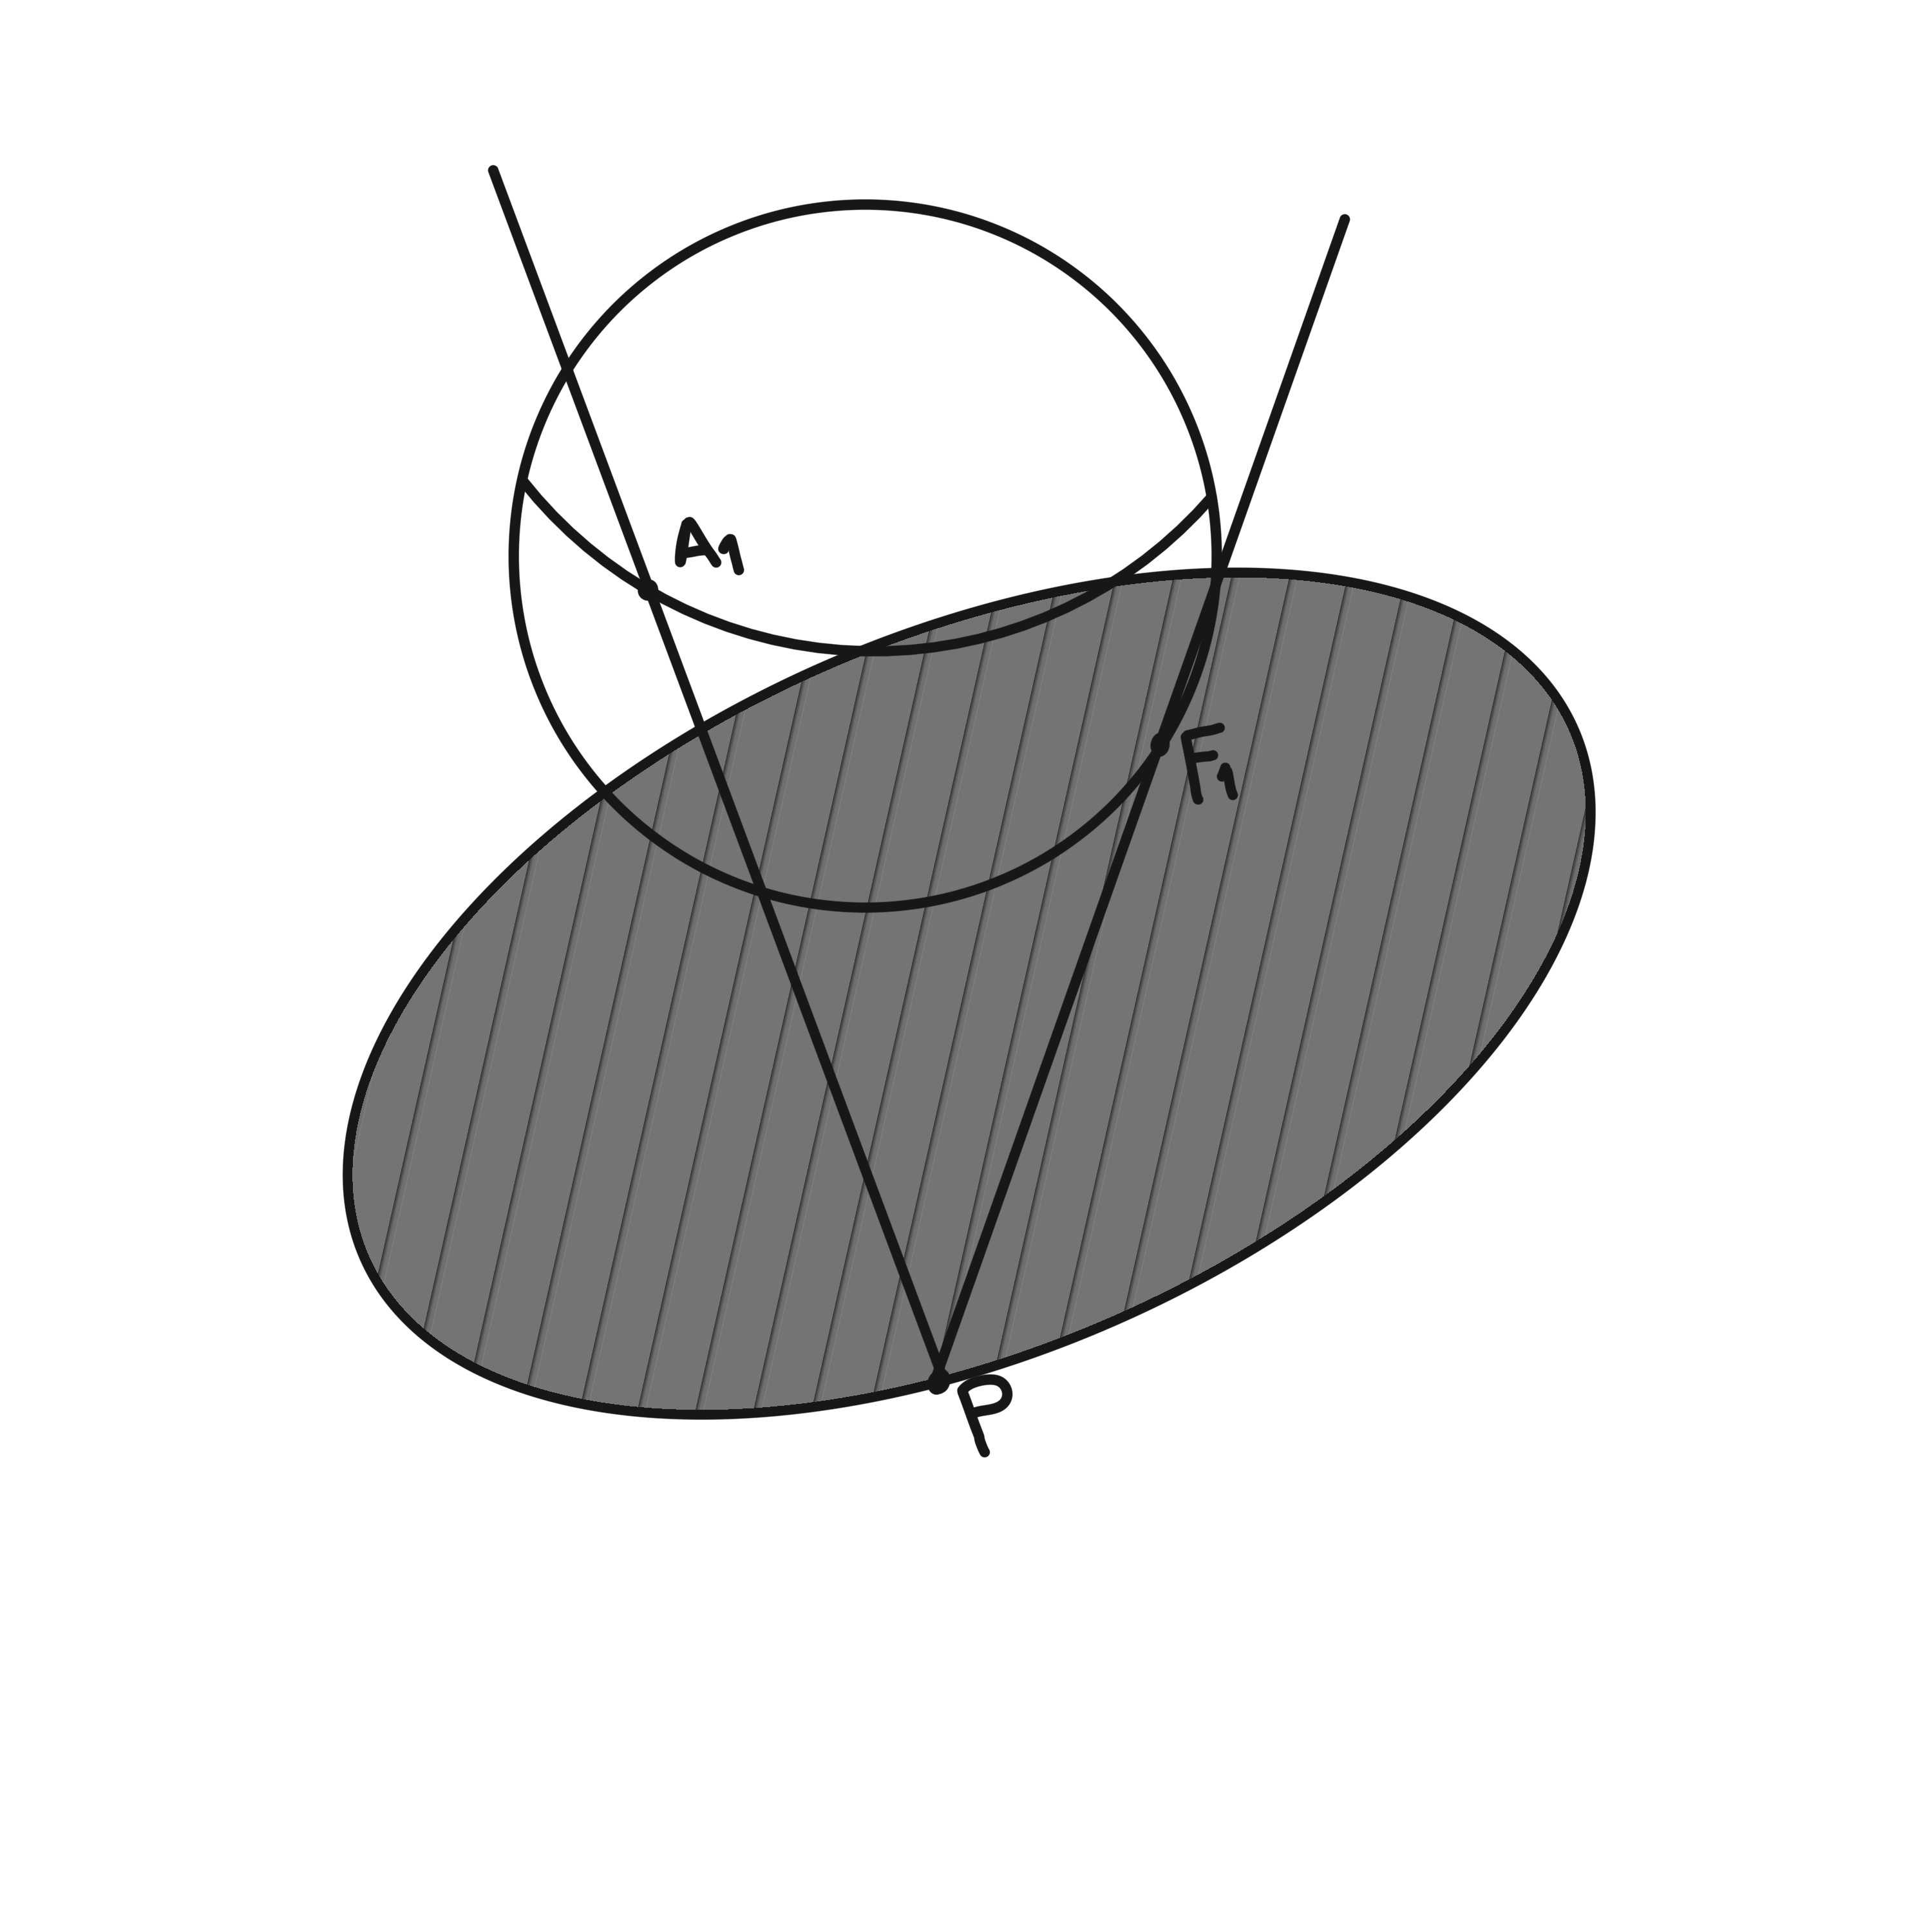
\includegraphics[width=\textwidth]{ez.png}
          \caption{\(\left\lVert \vec{PF_1}  \right\rVert  = \left\lVert \vec{PA_1}  \right\rVert \)}
        \end{minipage}
        \hfill
        \begin{minipage}[b]{0.4\textwidth}
          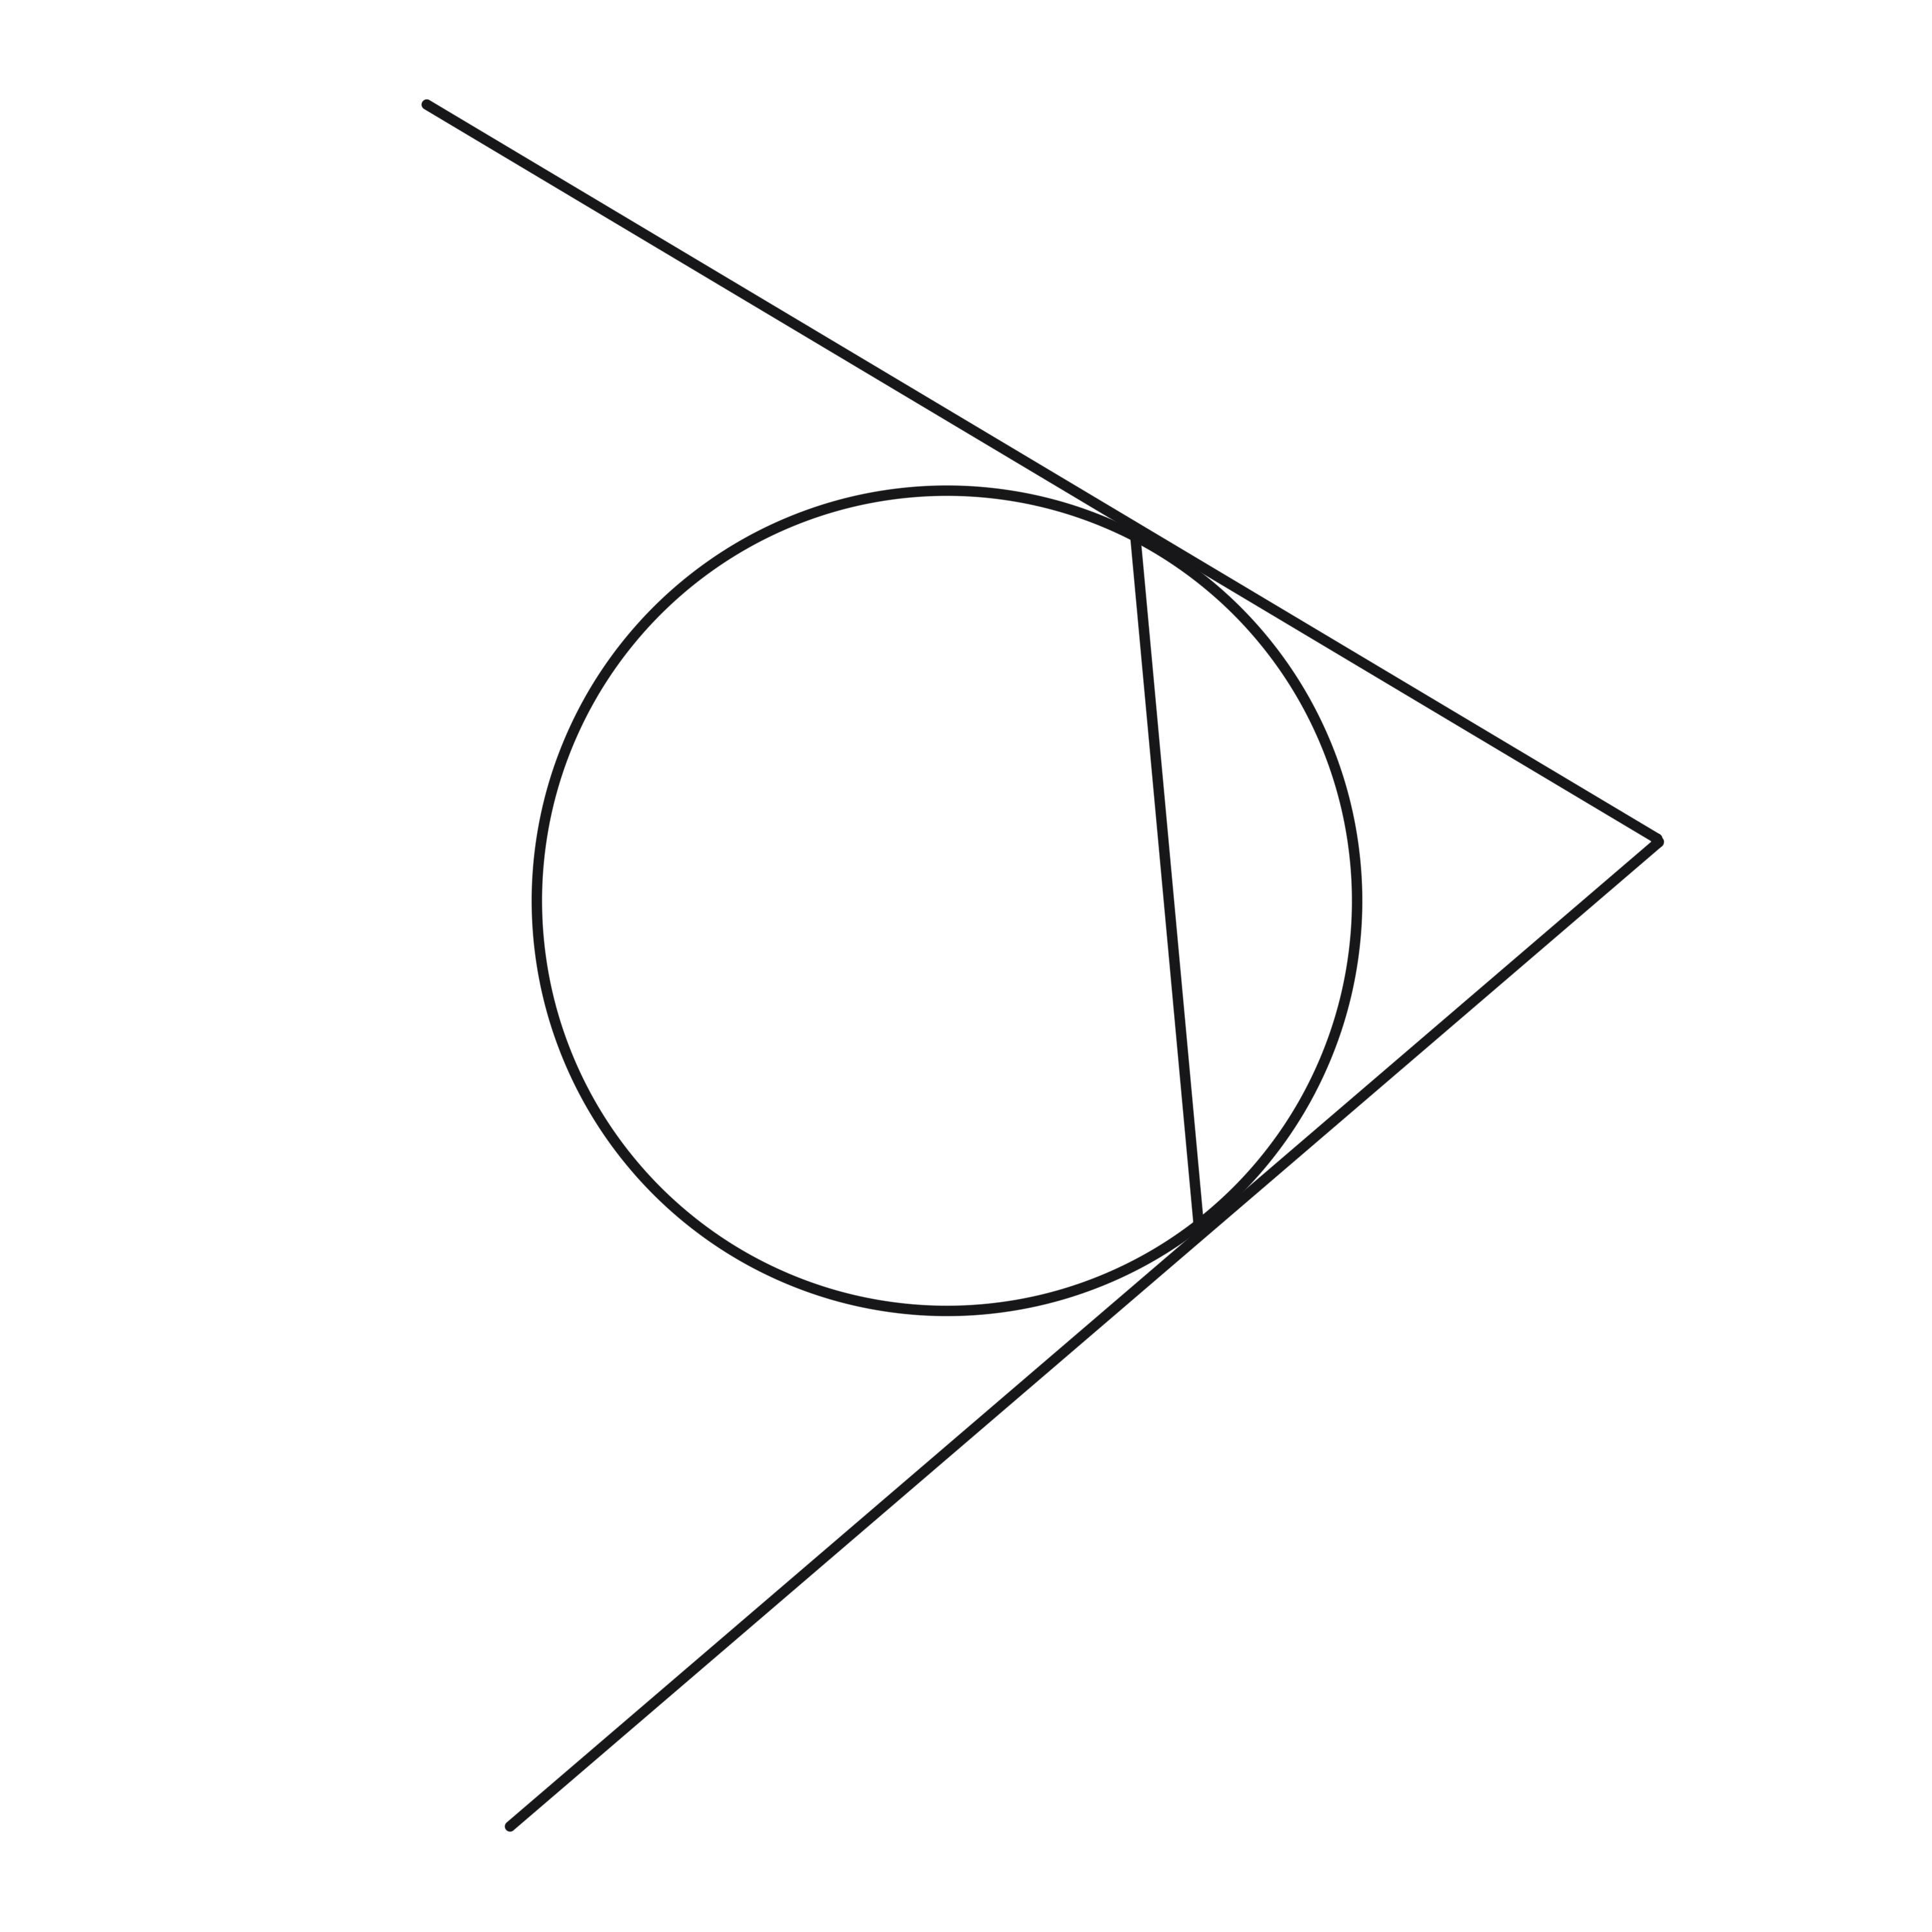
\includegraphics[width=\textwidth]{Untitled_4.png}
          \caption{Visualizzazione 2D punti di tangenza}
        \end{minipage}
      \end{figure}

      \subsection{Equazione cartesiana dell'ellisse}
scegliendo un sistema di riferimento appropriato, a partire dalla caratterizzazione dell'ellisse come luogo geoemtrico, è possibile scrivere la sua eq.cartesiana in forma canonica.
\\
Un'ellisse ha due assi di simmetria: l'asse maggiore ( o focale) e l'asse minore. Il punto d'intersezione 0 degli assi È il centro di simmetria. I punti di intersezioen tra l'ellisse e gli assi cartesiani sono i vertici di esso.
\\
Consideriamo un ellisse \( \xi  \) con fuochi \(F_1 e F_2\) e indichiamo con 2c la loro distanza. scegliamo gli assi cartesiani in modo che coincidano con gli assi di simmetria. 

%aggiungere grafico ellisse

\( P(x,y) \in \xi \Longleftrightarrow \left\lvert PF_1 \right\rvert + \left\lvert PF_2 \right\rvert = 2a \, \, a > c \) 









\end{document}